\makeatletter
\def\input@path{{../../}}
\makeatother
\documentclass[../../main.tex]{subfiles}

\graphicspath{
	{../../img/}
	{../img/}
	{img/}
}

\begin{document}
\section{Комплекснозначные функции действительного переменного (КФ). 
Множество на комплексной плоскости}

\emph{Комплекснозначной функцией действительного переменного} (КФ) будем 
называть произвольное отображение: 
\begin{equation}
\label{lec25:1}
f: [\alpha,\beta ] \longrightarrow \C, \ \text{где}\;[\alpha,\beta ] \subset \R.
\end{equation}
В соответствии с \eqref{lec25:1} для 
$ \forall t \in  [\alpha,\beta ]\  \exists! f(t) \in \C$. Представим $f(t)$ в
параметрическом виде:
\begin{equation}
\label{lec25:2}
f(t) = x(t) + i y(t),\ \text{где}\  \begin{cases}
	x(t) = \operatorname{Re} f(t) \in \R \\
	y(t) = \operatorname{Im} f(t) \in \R
           \end{cases}.
\end{equation}
\begin{exmp}
\[
\begin{cases}
	z_0 = x_0 +  iy_0 \\
	x_0, y_0 \in \R
\end{cases}
\]

Пусть $r \in \R, \ r > 0$ --- некоторое число. Тогда
$ |z - z_0| = r$ соответствует множеству точек, равноудалённых
на расстояние $r$ от $z_0$ $\implies$ окружности с центром в $z_0$
 и радиусом $r$.
$|z -z_0| = \sqrt{(x-x_0)^2 + (y - y_0)^2} 
\implies (x-x_0)^2 + (y - y_0)^2 = r^2$.
Эту окружность можно параметризовать следующим
образом:
\[
\begin{cases}
	x = x_0 +  r\cos{t} \\
	 y=  y_0 + r\sin{t}
\end{cases} \quad t \in [-\pi, \pi].
\]
\[
\begin{cases}
	x = x_0 +  r\cos{t} \\
	 y=  y_0 + r\sin{t}
\end{cases} \implies z = x+ iy = x_0 + iy_0 + r(\cos{t} + i\sin{t}) = z_0 + r{e}^{it}
\]

Таким образом, получим следующую КФ:
\[
\begin{cases}
	f(t) = z_0 + r{e}^{it} \\
	\quad t \in [-\pi, \pi]
\end{cases}.
\]
\end{exmp}

\hfill

Для КФ \eqref{lec25:1},\eqref{lec25:2}  все основные свойства определяются
через функции $x(t)$ и $y(t)$ как действительные Ф1П.
\[
\lim\limits_{t \to t_0}  f(t) = P = A + iB \in \C \iff
\begin{cases}
	\lim\limits_{t \to t_0}  x(t)  = \operatorname{Re} P = A \in \R \\
	\lim\limits_{t \to t_0}  y(t)  = \operatorname{Im} P = B \in \R
\end{cases} 
\]
Из чего следует, что  все основные свойства сходящихся Ф1П 
(кроме свойств, использующих неравенства),
арифметические операции над сходящимися Ф1П автоматически переносятся на КФ.
В частности, функция \eqref{lec25:1} непрерывна в $t_0 \in [\alpha,\beta ]$,\   если 
$\exists \lim\limits_{t \to t_0}  f(t) = f(t_0) \iff 
\begin{cases}
	\lim\limits_{t \to t_0}  x(t)  = x(t_0) \\
	\lim\limits_{t \to t_0}  y(t)  =  y(t_0)
\end{cases}$.

КФ будем считать дифференцируемой в $t_0 \in [\alpha,\beta ]$,\   если 
$\begin{cases}
	\exists x'(t)  \in \R \\
	\exists y'(t)  \in \R
\end{cases}$. Производную КФ будем определять следующим образом:
\[
	f'(t) = x'(t) + iy'(t) \in \C
\]

Если $f(t)$ дифференцируема $t_0 \in E \subset [\alpha,\beta ]$, 
то она считается дифференцируемой на $E$ (на концах 
подразумевается односторонняя дифференцируемость,
определемая как существование соответствующих 
односторонних производных для $x(t), \ y(t)$).

Если $\begin{cases}
	\exists \int\limits_{\alpha}^{\beta} x(t)\;dt  \in \R \\
	\exists \int\limits_{\alpha}^{\beta} y(t)\;dt  \in \R
\end{cases}$, то по определению полагаем
$\int\limits_{\alpha}^{\beta} f(t)\;dt = 
\int\limits_{\alpha}^{\beta} x(t)\;dt + i\int\limits_{\alpha}^{\beta} y(t)\;dt$.
Интегрируемые КФ (и интегралы КФ) обладают
основными свойствами, аналогичными 
свойствам интегрируемых Ф1П (и ОИ).
\begin{exmps}\  
\begin{enumerate}
\item\[\begin{cases}
	f(t) = e^{iat} \\
	a = const \in \R
\end{cases}\!\! t \in [\alpha, \beta]
\qquad
\eqref{lec25:2} \iff 
\begin{cases}
	x(t) = \cos{at} \\
	y(t) = \sin{at}
\end{cases}  
\]
\[\begin{cases}
	\exists x'(t) = -a\sin{at}  \\
	\exists y'(t) = a\cos{at}
\end{cases}\implies \exists \left(e^{iat} \right)' = -a\sin{at} + ia\cos{at} =
 ia(\cos{at} + i\sin{at}) = iae^{iat}
\]
\item\[
\int\limits_{\alpha}^{\beta}e^{iat}\;dt =
\int\limits_{\alpha}^{\beta}e^{iat}\cos{at}\;dt +
 i\int\limits_{\alpha}^{\beta}\sin{at}\;dt = 
 \frac{\sin{a\beta} - \sin{a\alpha}}{a}\quad  - \quad  
 i\ \frac{\cos{a\beta} - \cos{a\alpha}}{a} = \]\[
= \left[ \frac{-i{e}^{iat}}{a} \right]_{\alpha}^{\beta}= 
\left[ \frac{{e}^{iat}}{ia} \right]_{\alpha}^{\beta}
\]
\end{enumerate}
\end{exmps}

\begin{wrapfigure}{r}{0.4\textwidth}
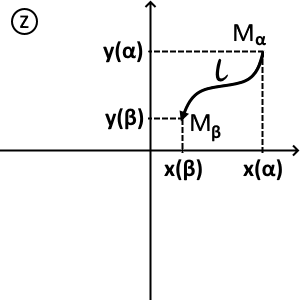
\includegraphics[width=0.4\textwidth]{lec25_1.png}
\end{wrapfigure}
На комплексной плоскости \textcircled{z}\  КФ \eqref{lec25:2} соответствует
некоторая кривая $l$, ограниченная точками \  $
\begin{cases}
	M_{\alpha} = (x({\alpha}, y{\alpha}) \\
	M_{\beta} = (x({\beta}, y{\beta})
\end{cases} $. Движение от $M_{\alpha}$ к $M_{\beta}$ будем называть 
\emph{положительным}. Таким образом мы получили положительно
определённую кривую $l^+$. Аналогично определяем отрицательную
кривую $l^-$.

Если  $M_{\alpha} = M_{\beta}$, то кривая $l$ будет замкнута. 
Замкнутую кривую  $l$ будем называть \emph{замкнутым контуром},
если $l$ не имеет самопересечений и функция непрерывна. В общем
случае, замкнутую кривую  $l$ с движением против часовой стрелки
будем называть \emph{положительно ориентированной}, 
а по часовой ---
\emph{отрицательно ориентированной}. По аналогии  с $\R^2$,
 на комплексной плоскости  \textcircled{z} \ будем рассматривать 
следующие  простейшие множества:

Пусть $\fix{z_0}\in \C, k>0\ \in \R$
\begin{enumerate}
\item Окружность: \[  |z - z_0| = k\] 
\item Замкнутая $k$-окрестность $z_0$ : \[ |z - z_0| \leq k\] 
\item Открытая $k$-окрестность $z_0$ : \[ |z - z_0| < k\] 
\end{enumerate}
\end{document}
